% Note that if you want something in single space you can go back and
% forth between single space and normal space by the use of \ssp and
% \nsp.  If you want doublespacing you can use \dsp.  \nsp is normally
% 1.5 spacing unless you use the doublespace option (or savepaper
% option)
%
%(FORMAT) usually you *don't* want to mess with the spacing for your
%(FORMAT) final version.  If you think/know that the thesis template
%(FORMAT) and/or thesis style file is incorrect/incomplete, PLEASE
%(FORMAT) contact the maintainer.  THANK YOU!!!

\chapter{COMPUTATIONAL GEOMETRY}
\label{chap:intro}
% By labeling the chapter, I can refer to it later using the
% label. (\ref{chap:intro}, \pageref{chap:intro}) Latex will take care
% of the numbering.

\section{Introduction}

The easiest explanation of geometric algorithms is what a software developer programs to solve geometry problems. And we all know what geometry problems are, right?  The simplest of such problems might be to find the intersection of two lines, the area of a given region, or the inscribed circle of a triangle.  Methods and formulas have been around for a long time to solve such simple problems.  But, when it comes to solving even these simple problems as accurate, robust, and efficient software programs, the easy formulas are sometimes inappropriate and difficult to implement.  This is the starting point for geometry algorithms as methods for representing elementary geometric objects and performing the basic constructions of classical geometry.

Recently, a new extension of geometry, now referred to as ``computational geometry",  has arisen that goes beyond the scope of classical geometries.  This extension has been made possible by, and has emerged from, modern computer technology.  In short, this brand of geometry is interested in massive problems with many objects (such as large sets of points or lines). Computational geometry is a branch of computer science dedicated entirely to the study of geometric algorithms and its applications in computer science. The size of the computational problem is measured by the size `n' of the large set of objects involved.  A major concern of computational geometry is to determine algorithms that are: 
\begin{enumerate}
\item efficient even when the problem's size gets larger and larger; 
\item practical and efficient for reasonably sized problems; and 
\item accurate and robust on finite state computing machines.
\end{enumerate}

It is somewhat inappropriate to refer to the solving of such massive geometry problems as ``computational", and this has created some confusion.  In fact, classical geometry algorithms can involve more direct computation using established formulas, whereas this new brand of computer geometry is more algorithmic in nature, depending as much on the organization of the steps it performs as the actual mathematics used \cite{SOFTSURFER}.
 
There are many useful and interesting applications of computational geometry, some of which include robotics, computer graphics, computer aided design (CAD), computer aided manufacturing (CAM) and geographic information science (GIS) among many others (Appendix~A). Computational geometry emerged in the late 1970s and has grown tremendously since then. There are many active research programs being conducted in this area of computer science attracting a large number of students and companies. Having been working as a software developer in the leading GIS software company, Environmental System Research Institute (esri), I recognize the importance of this subject and the role it plays in practical applications. I have personally seen many groups working hard to understand and implement various algorithms in computational geometry. These algorithms have tremendously helped in solving some of the real world problems which have made this world a better place to live in.

It has been noted that there is nothing new about viewing geometry as algorithmic.  In fact, much of Euclid's geometry consists of algorithms to perform geometric constructions using basic operations with a straightedge and compass.  It�s just that the problems were smaller since the Greek computing machine was an actual engineer using these implements to achieve the construction, and his speed was at best several operations per minute.  Modern computers can do billions of operations per second, and so the door is now open to devise algorithmic procedures for solving large scale geometric problems \cite{SOFTSURFER}.

\section{Research Objective}
The research objective of this thesis is to study one algorithm in Computational Geometry namely the ``Line Sweep Algorithm" and present a working copy of it which can be useful for future students/ researchers. Also I would be proposing a slight modification in one of the data structures used in the algorithm with an intent to optimize it's execution time. I will then compare the traditional algorithm with the modified one to see if we have achieved any success in optimizing it.

\section{Applications}

There is a good recent (1996) Task Force Report ``Application Challenges to Computational Geometry" \cite{TaskForeReport} describing many modern applications of algorithmic geometry.  It notes that with the explosion in computer graphics technology, ``geometric computing is creeping into virtually every corner of science and engineering".  One could add business and finance, education, entertainment to the list.  

\subsection{Computer Graphics and Imaging}

Computer graphics generally involves the drawing of 2-dimensional and 3-dimensional objects on computer screen, printer, plotter or any other digital surface. Typical problems in computer graphics which involve the usage of computational geometry are computing intersections of geometric objects, transformation in co-ordinate system, extrusion of objects, finding the relative position of an object with respect to the mouse, etc. Computer Graphics and Imaging uses geometry algorithms to represent, render, and visualize complex real and virtual worlds, such as we often see in recent movies, video games, or training simulators.  Basic methods include geometric modeling, clipping, set operations, space partitions, point location, etc.  Advanced techniques include visibility determination (hidden surface removal, ray tracing), shadow casting, radiosity and collision detection.

\subsection{Robotics}

Robotics involves the study of design and implementation of robots. Use of computational geometry is pretty much obvious in the field of robotics since robot operate in the real world (3-dimensional). Hence at each and every step of robotic development there is some contribution of computational geometry such as calculation of accurate placement of a robot arm, the angle in which to rotate the robot arm in order to perform a specific task, finding out the shortest path from point A to point B while avoiding obstacles (Figure.~\ref{fig1} \cite{ROBOT}). This involves both obstacle collision avoidance and minimal route planning (perhaps with other geometric constraints, like terrain slope).  Problems involve geometry algorithms for moving polytope objects past polytope obstacles.  The robots involved can be used for industrial purposes, or can be fully or semi-autonomous vehicles.  For example, autonomous robots we send to other planets will need to have computer vision for reconstructing scene geometry models which are then used for exploratory motion planning. I personally have coded a genetic algorithm to find the optimum path of a robot to move from point A to point B where the robot learns about obstacles based on the sensors placed in front of them. Thus it was a real time algorithm which adapted itself based on the obstacles it learns as it moves forward.
\begin{figure}[ht]
  \begin{center}
   	\fbox{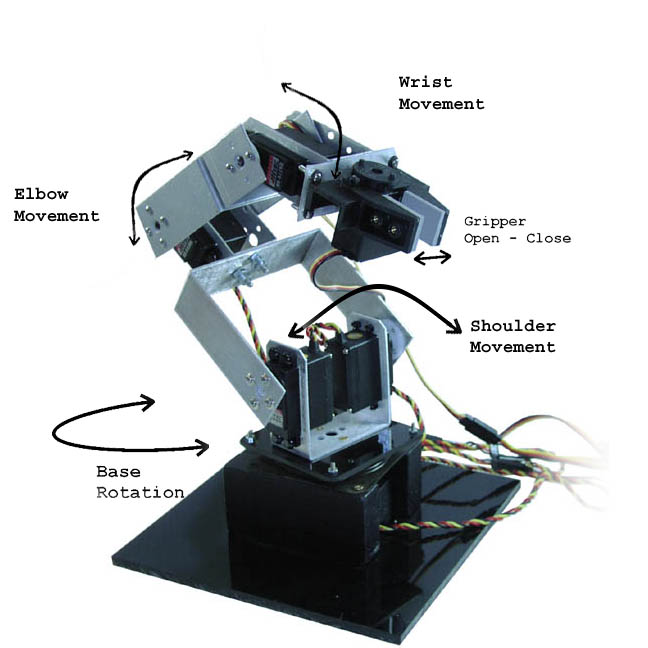
\includegraphics[width=3.5in, height=4.5in]{Figures/Figure1}}
  \end{center}
  \centering
	\parbox{3.5in}{\caption{Robotic arm movement. Source: IMAGESSI, \textbf{\textit{Robotic arm kit}}. Images Scientific Instruments,
http://www.imagesco.com/kits/robotic-arm.html, accessed Aug. 2012, n.d.} \label{fig1}} 
\end{figure}

\subsection{Manufacturing and Product Design}

Computer-aided design (CAD), also known as computer-aided design and drafting (CADD), \cite{CAD} is the use of computer systems to assist in the creation, modification, analysis, or optimization of a design \cite{CAD1}. In simple terms, it means the design of products using computer technology before they are actually manufactured. These products can be of any type, including Lego blocks, automobile machinery, furniture, spare parts, dyes etc. Since these are real world objects, computational geometry obviously plays a major role in the design of these products, their alignment with respect to each other, their shape and how each part would fit into each other. Computer-aided manufacturing (CAM) is the use of computer software to control machine tools and related machinery in the manufacturing of workpieces \cite{CAM3, CAM2, CAM4, CAM5, CAM1}. In short it involves the actual manufacturing of the design or prototype built using CAD packages. CAM also involves many challenges for geometric algorithms, especially assembly decisions and testing of the manufactured product. 

\subsection{Molecular Biology}

Molecular Biology has a high demand for geometry algorithms to model and analyze large scale molecular models associated with proteins, DNA, etc.  The human genome project is producing more-and-more data every day, and using it to produce and investigate models of the basis of life and evolution is an enormous challenge.  Even at the rudimentary level of cellular mechanisms, breakthroughs in geometric modeling and understanding may be the key to finding cures for genetic diseases.  A specific promising problem is to model the spatial structure of proteins, and use this to design drugs that geometrically bind with their receptors \cite{SOFTSURFER}.

In this research thesis, geometric algorithms are considered primarily in the context of GIS applications. This focus of my research comes in part because I have a few years of experience working in the GIS field. A geographic information science (GIS) integrates hardware, software, and data for capturing, managing, and displaying all forms of geographically referenced information. GIS allow us to view, understand, question, interpret, and visualize data in many ways that reveal relationships, patterns, and trends in the form of maps, globes, reports, and charts. A GIS helps you answer questions and solve problems by looking at your data in a way that is quickly understood and easily shared \cite{esriDef}. Answering these geographic questions is not a trivial task and often requires detailed understanding of the algorithms required to solve these problems. Geometric algorithms are heavily used in this area and are typically included as a geo-processing tool in most of the GIS software.

To give a simple example, consider that Starbucks coffee chain wants to open a new store in the state of California. The company will want to determine the optimum location as a function of numerous variables characterizing the available physical space and the socioeconomic demographics around it. This process, if done manually by a person with expertise, can literally take many days and even weeks to produce a correct answer. This task can be completed in a few minutes with the help of the right geo-processing tools, which internally implement computational geometric algorithms (for example the Voronoi diagram). Some of the variables this tool would take into consideration are the population density, average income, proximity of existing stores, other competing stores, etc. These algorithms must be made as efficient as possible because they typically operate on huge datasets and do many complex calculations for each item.

These are some of the areas in which geometry algorithms play a critical role.  Since everything we see and touch has a geometric aspect enabling us to understand our world, and the computer graphics and geometry ball is on the roll and gaining momentum, more-and-more areas of endeavor will start to be influenced by geometry algorithms.  You will recognize them when you see them.  But, will you know the best algorithms for new areas of application?  Knowing the fundamentals, and the scope of our current knowledge will help.
